\documentclass[serif, mathserif, professionalfont]{beamer} % Remove notes for no notes
%\documentclass[notes]{beamer}       % print frame + notes
%\documentclass[notes=only]{beamer}   % only notes
%\documentclass{beamer}              % only frames
\usetheme{BlueGrey}
\usenavigationsymbolstemplate{}
\renewcommand{\newblock}{}
\setlength{\parskip}{1em}

\usepackage{natbib}
\bibliographystyle{apalike}%plainnat}

\usepackage{bm}
\usepackage{xmpmulti}
\usepackage{amsmath}
\usepackage{amssymb}
\usepackage{palatino}
\usepackage{graphicx}
\usepackage{subfigure}
\usepackage{relsize}
\usepackage{setspace}
\usepackage{pxfonts}
\usepackage{multicol}
\usepackage{color}
\usepackage{tikz,pgfplots}
\usepackage{comment}
\usepackage{cancel}
\usetikzlibrary{pgfplots.groupplots}
\usetikzlibrary{plotmarks}
\pgfplotsset{compat=newest}
\pgfplotsset{filter discard warning=false}
\usepgfplotslibrary{groupplots}
\definecolor{english}{rgb}{0.0, 0.5, 0.0}
\definecolor{ballblue}{rgb}{0.13, 0.67, 0.8}
\input{definitions.tex}
\input{notationDef.tex}

\newcommand{\fV}{\mappingFunctionVector}
\newcommand{\yV}{\dataVector}
\newcommand{\noiseVar}{\dataStd^{2}}
\newcommand{\xV}{\inputVector}
\newcommand{\Wmat}{\bm{W}}
\newcommand{\Cmat}{\bm{C}}
\newcommand{\muV}{\bm{\mu}}
\newcommand{\sigmaV}{\bm{\sigma}}
%\newcommand{\likVar}{\beta^{-1}}

%\definecolor{intract}{rgb}{0.227, 0.038, 0.54}
\definecolor{intract}{RGB}{227, 38, 54}
\definecolor{tract}{RGB}{86, 130, 3}

\title{Non-Gaussian likelihoods for Gaussian Processes}
\author{Alan Saul}
\institute{University of Sheffield}
\date{}

\begin{document}
%\frame{
%\begin{center}
    %{\huge Non-Gaussian likelihoods for Gaussian Processes}\\
    %\vspace{2em}
    %Alan Saul\\
    %University of Sheffield\\
    %\vspace{2em}
    %%\includegraphics[width=0.4\textwidth]{../../../logo_sheff}
%\end{center}
%}
\frame{\titlepage}

\frame{
\frametitle{Outline}
    \begin{itemize}
        \item Motivation
        \item Laplace approximation
        \item KL method
        \item Expectation Propagation
        \item Comparing approximations
    \end{itemize}
}
\note{
    Motivation:
        What is a likelihood?
        non-Gaussian likelihoods, examples, 
        Bernoulli, Student-T, Poisson
        True posterior approximation not possible, all the following methods look at approximating this true posterior with a Gaussian distribution in some way.
        Once we have a Gaussian approximation to the posterior, we can use it as normal, for example making predictions etc.
        Many ways in which we could approximate the distribution, approximate around shape of a single mode, approximate overall density, should we care more about capturing density of leaving it out if we have to choose?
        Show an overview of how the different methods might approximate different distributions
    Laplace approximation
        Find the mode of the true posterior distribution
        Do a taylor expansion around this point, which finds the curvature around this point
        Approximate with a Gaussian with this mean and the same curvature
    KL method
        We say we have a Gaussian distribution, whos parameters we can tweak to match the shape of the posterior
        We define a similarity measure between our Gaussian distribution, and the true posterior, this is the KL.
        KL is the average additional amount of information required to specify the values of $f$ as a result of using an approximate distribution $q(f)$ instead of the true distribution, $p(f|y)$.
        It is not a symmetrical quantity and is always zero or positive (we must provide some additional information, or no information at all).
        Show some examples of how the KL changes for different likelihoods, maybe a convolution
        We can't compute the KL divergence between the true posterior and the approximate posterior, as it requires integrating over a quantity we can't compute directly?
        The trick is to try and minimize the $KL[q(f|y)||p(f|y)]$, by forming a lower bound on the marginal likelihood which we will in turn maximise
        This needs lots of figures!
        Leads to distributions $q(f)$ that avoid regions of $p(f|y)$ that have low density (heavily penalized for putting density where there is little)
    Expectation Propagation
        This is a more algorithmic approach to making the approximation. Shown to be the most effective method for the classification likelihood.
        Looks at approximating the true posterior with a product of site-approximations (Gaussian distributions).
        These site distributions are -not- Gaussian approximations to each likelihood component, but overall make the marginal likelihood similar to true marginal
        Iterative procedure, give outline
        Moment match - set the mean and variances of the two distributions to be equal
        Although for EP the KL divergence is only for each of the marginals individually $KL[p(f_i|y_i)||q(fi)]$, not the full KL divergence $KL[p(f|y)||q(f)]$, this KL divergence is minimized when density is assigned by $q(fi)$ to regions where $p(fi|yi)$ has density (heavily penalized for not putting density where there is lots)
    Overall properties, when to use which?
        Laplace approximation 
            Pros - Very fast
            Cons - Poor approximation if the mode does not well describe the posterior, for example Bernoulli likelihood (probit)
                 - As a result it can assign lots of density to areas where there is none
            When - When the posterior is well characterized by its mode, for example Poisson.
        KL method
            Pros - Can be relatively quick, and lends it self to sparse approximations
                 - Principled in that it we are directly optimizing a measure of similarity between an approximation and true distribution
            Cons - 
            When - When the we 
        EP method
            Pros - Very effective for certain likelihoods (classification)
            Cons - Slow though possible to extend to sparse case. 
                 - Convergence issues for certain likelihoods
                 - Must be able to match moments
            When -
        MCMC methods
            If accuracy is key, it is also possible to use a range of different sampling techniques
            These have a tendency to be very slow though in the limit of infinite samples, they are theoretically exact.
        \cite{Approximations for Binary Gaussian Process Classification}
    Bonus
        Heteroscedastic likelihoods
}

\frame{
    \frametitle{GP regression}
    \begin{overprint}
    Model the observations as a distorted version of the process $\fV_{i}$:
    \begin{equation*}
        \yV_{i} \sim \gaussianSamp{f(\xV_{i})}{\noiseVar}
        %\yV_{i} \sim \gaussianDist{\yV_{i}}{f(\xV_{i})}{\noiseVar}
    \end{equation*}
    $f$ is a non-linear function, in our case we assume it is latent, and is assigned a Gaussian process prior.
    \end{overprint}
    \begin{overprint}
        \centerline{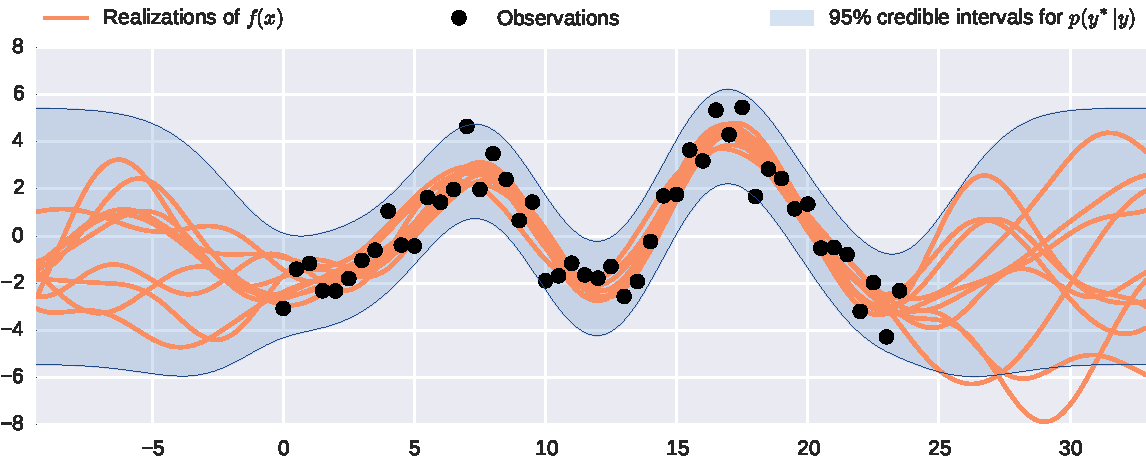
\includegraphics[width=1\textwidth]{../diagrams/PosteriorGP.pdf}}
    \end{overprint}
}

\frame{
    \frametitle{GP regression setting}
    So far we have assumed that the latent values, $\fV$, have been corrupted by Gaussian noise.
    Everything remains analytically tractable.
    \begin{align*}
        \text{Gaussian Prior:} & & \fV \sim \mathcal{GP}(\zerosVector, \Kff) = p(\fV)\\
        \text{Gaussian likelihood:} & & \yV \sim \gaussianSamp{\fV}{\noiseVar\eye} = \prod^{\numData}_{i=1} p(\yV_{i}|\fV_{i})\\
        \text{Gaussian posterior:} & & p(\fV|\yV) \propto \gaussianDist{\yV}{\fV}{\noiseVar\eye}\gaussianDist{\fV}{\zerosVector}{\Kff}
    \end{align*}
}

\frame{
    \frametitle{Likelihood}
    \begin{itemize}
        \item $p(\yV|\fV)$ is the probability of the observed data, if we know the latent function values $\fV$.
        \item Can also be seen as the likelihood that the latent function values, $\fV$, would give rise to some observed data, $\yV$.
        \item So far assumed that the distortion of the underlying latent function, $\fV$, that gives rise to the observed data, $\yV$, is independent and Gaussianly distributed.
        \item This is often not the case, count data, binary data, etc.
    \end{itemize}
}

\frame{
    \frametitle{Binary example}
    \begin{itemize}
        \item Binary outcomes for $\yV_{i}$, $\yV_{i} \in [0,1]$.
        \item Model the probability of $\yV_{i} = 1$ with transformation of GP.
        \item Probability of $1$ must be between $0$ and $1$, thus use squashing transformation, $\lambda(\fV_{i}) = \Phi(\fV_{i})$.
    \end{itemize}
    \begin{align*}
        \yV_{i} = \left\{
            \begin{array}{ll}
                1, & \text{with probability $\lambda(\fV_{i})$.}\\
                0, & \text{with probability $1-\lambda(\fV_{i})$.}
            \end{array}
        \right.
    \end{align*}
    \centerline{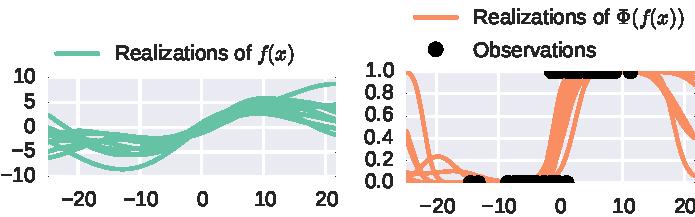
\includegraphics[width=1.0\textwidth]{../diagrams/BernoulliPosterior.pdf}}
}

\frame{
    \frametitle{Count data example}
    \begin{overprint}
    \begin{itemize}
        \item Non-negative and discrete values only for $\yV_{i}$, $\yV_{i} \in \mathbb{N}$.
        \item Model the \emph{rate} or \emph{intensity}, $\lambda$, of events with a transformation of a Gaussian process.
        \item Rate parameter must remain positive, use transformation to maintain positiveness $\lambda(\fV_{i}) = \exp(\fV_{i})$ or $\lambda(\fV_{i}) = \fV_{i}^2$
    \end{itemize}
    \begin{align*}
        \yV_{i} \sim \text{Poisson}(\yV_{i}|\lambda_{i} = \lambda(\fV_{i}))\quad\quad
        \text{Poisson}(\yV_{i}|\lambda_{i}) = \frac{\lambda_{i}^{\yV_{i}}}{!\yV_{i}}e^{-\lambda_{i}}
    \end{align*}
\end{overprint}
\begin{overprint}
    \centerline{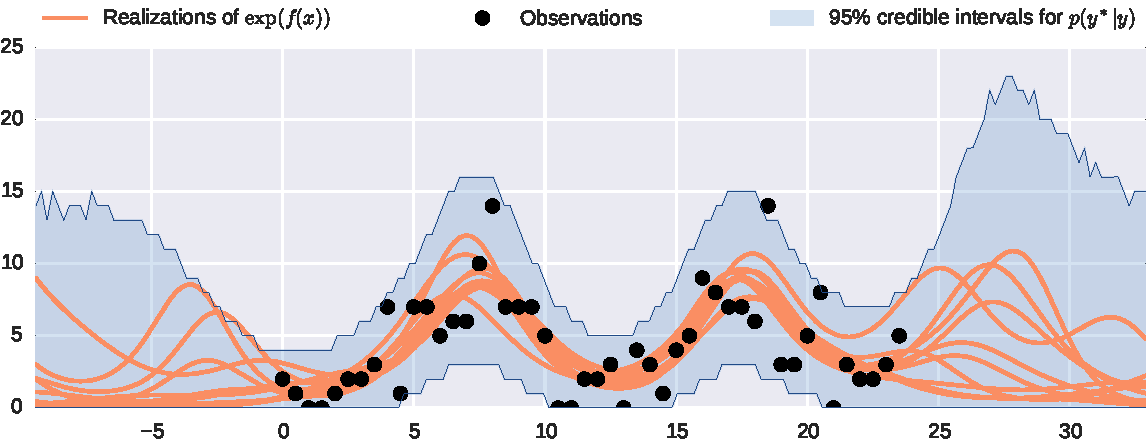
\includegraphics[width=.9\textwidth]{../diagrams/PoissonPosterior.pdf}}
\end{overprint}
}


\frame{
    \frametitle{Non-Gaussian posteriors}
    \begin{itemize}
        \item Exact computation of posterior is no longer analytically tractable due to non-conjugate Gaussian process prior to non-Gaussian likelihood, $p(\yV|\fV)$.
    \end{itemize}
    \begin{equation*}
        {\color{intract}p(\fV|\yV)} = \frac{p(\fV)\prod^{\numData}_{i=1}p(\yV_{i}|\fV_{i})}{\color{intract}\int p(\fV)\prod^{\numData}_{i=1}p(\yV_{i}|\fV_{i})\,d\fV}
    \end{equation*}
    \begin{itemize}
        \item Various methods to make a Gaussian approximation, $q(\fV) \approx {\color{intract}p(\fV|\yV)}$.
        \item Allows simple predictions 
    \end{itemize}
    \begin{align*}
        p(\fV^{*}|\yV) &= \int p(\fV^{*}|\fV){\color{intract}{p(\fV|\yV)}} d\fV\\
                       &\approx \int p(\fV^{*}|\fV)q(\fV) d\fV
    \end{align*}
}

\frame{
    \frametitle{Laplace approximation}
    \begin{itemize}
        \item Find the mode of the true log posterior, via Newton's method.
        \item Use second order Taylor expansion around this modal value.
            \begin{itemize}
                \item i.e obtain curvature at this point.
            \end{itemize}
        \item Form Gaussian approximation setting the mean equal to the posterior mode, $\hat{\fV}$, and matching the curvature.
        \item ${\color{intract}p(\fV|\yV)} \approx q(\fV|\muV,\Cmat) = \gaussianDist{\fV}{\hat{\fV}}{(\Kff^{-1} + \Wmat)^{-1}}$
        \item $\Wmat \triangleq -\frac{d^{2}\log p(\yV|\hat{\fV})}{d\hat{\fV}^{2}}$.
        \item For factorizing likelihoods (most), $\Wmat$ is diagonal.
    \end{itemize}
}
\note{The actual optimization is in log space, but here we show the result in the distribution space}

\frame{
    \frametitle{Visualization of Laplace}
    %\animategraphics[controls]{1}{../diagrams/laplace-anim}{0}{6}
    \multiinclude[<+>][format=pdf,graphics={scale=0.4}]{../diagrams/laplace-anim}
}

\frame{
    \frametitle{KL-method}
    \begin{itemize}
        \item Make a Gaussian approximation, $q(\fV) = \gaussianDist{\fV}{\muV}{\Cmat}$, as similar possible to true posterior, ${\color{intract}p(\fV|\yV)}$.
        \item Treat $\muV$ and $\Cmat$ as variational parameters, effecting quality of approximation.
        \item Define a divergence measure between two distributions, KL divergence, ${\color{intract}\KL{q(\fV)}{p(\fV|\yV)}}$.
        \item Minimize this divergence between the two distributions~\citep{Nickisch:class08}.
    \end{itemize}
}

\frame{
    \frametitle{KL divergence}
    \begin{itemize}
        \item General for any two distributions $q(\xV)$ and $p(\xV)$.
        \item $\KL{q(\xV)}{p(\xV)}$ is the average additional amount of information required to specify the values of $\xV$ as a result of using an approximate distribution $q(\xV)$ instead of the true distribution, $p(\xV)$.
        \item $\KL{q(\xV)}{p(\xV)} = \expectationDist{\log \frac{q(\xV)}{p(\xV)}}{q(\xV)}$
        \item Always 0 or positive, not symmetric.
        \item Lets look at how it changes with response to changes in the approximating distribution.
    \end{itemize}
}

\frame{
    \frametitle{KL varying mean}
    %\animategraphics[controls]{1}{../diagrams/KL_gaussian_mu}{0}{6}
    \multiinclude[<+>][format=pdf,graphics={scale=0.4}]{../diagrams/KL_gaussian_mu}
}

\frame{
    \frametitle{KL varying variance}
    %\animategraphics[controls]{1}{../diagrams/KL_gaussian_mu}{0}{6}
    \multiinclude[<+>][format=pdf,graphics={scale=0.4}]{../diagrams/KL_gaussian_var}
}

\frame{
    \frametitle{KL-method derivation}
    \begin{itemize}
        \item Assume Gaussian approximate posterior, $q(\fV) = \gaussianDist{\fV}{\muV}{\Cmat}$.
        \item True posterior using Bayes rule, ${\color{intract}p(\fV|\yV)} = \frac{p(\yV|\fV)p(\fV)}{p(\yV)}$.
        \item Cannot compute the KL divergence as we cannot compute the true posterior, $p(\fV|\yV)$.
    \end{itemize}
    \begin{align*}
        \color{intract}\KL{q(\fV)}{p(\fV|\yV)} &= \expectationDist{\log \frac{q(\fV)}{{\color{intract}p(\fV|\yV)}}}{q(\fV)}\\
                                               %&= \expectationDist{\log \frac{q(\fV)}{p(\fV)}p(\yV|\fV)p(\yV)}{q(\fV)}\\
                                               &= \expectationDist{\log \frac{q(\fV)}{p(\fV)} - \log p(\yV|\fV) + \log p(\yV)}{q(\fV)}\\
                                               &= \KL{q(\fV)}{p(\fV)} - \expectationDist{\log p(\yV|\fV)}{q(\fV)} + \log p(\yV)\\
        \log p(\yV) &= {\color{tract}\expectationDist{\log p(\yV|\fV)}{q(\fV)}} - {\color{tract}\KL{q(\fV)}{p(\fV)}} + {\color{intract}\KL{q(\fV)}{p(\fV|\yV)}}
    \end{align*}
}

\frame{
    \frametitle{KL-method derivation}
    \begin{align*} 
        \log p(\yV) &= {\color{tract}\expectationDist{\log p(\yV|\fV)}{q(\fV)}} - {\color{tract}\KL{q(\fV)}{p(\fV)}} + {\color{intract}\KL{q(\fV)}{p(\fV|\yV)}}\\
        &\geq {\color{tract}\expectationDist{\log p(\yV|\fV)}{q(\fV)}} - {\color{tract}\KL{q(\fV)}{p(\fV)}}
    \end{align*}
    \begin{itemize}
        \item Tractable terms give lower bound on $\log p(\yV)$ as $\color{intract}\KL{q(\fV)}{p(\fV|\yV)}$ always positive.
        \item Adjust variational parameters $\muV$ and $\Cmat$ to make tractable terms as large as possible, thus $\color{intract}\KL{q(\fV)}{p(\fV|\yV)}$ as small as possible.
        \item ${\color{tract}\expectationDist{\log p(\yV|\fV)}{q(\fV)}}$ with factorizing likelihood can be done with a series of $\numData$ 1 dimensional integrals.
        \item In practice, can reduce the number of variational parameters by reparameterizing $\Cmat = (\Kff - 2\Lambda)^{-1}$ by noting that the bound is constant in off diagonal terms of $\Cmat$.
    \end{itemize}
}

\frame{
    \frametitle{Expectation Propagation}
    \begin{align*}
        {\color{red}p(\fV|\yV)} &\propto p(\fV)\prod^{\numData}_{i=1}p(\yV_{i}|\fV_{i})\\
        q(\fV|\yV) &\triangleq \frac{1}{Z_{ep}}p(\fV)\prod^{\numData}_{i=1}t_{i}(\fV_{i}|\tilde{Z}_{i}, \tilde{\mu}_{i}, \tilde{\sigma}^{2}_{i}) = \gaussianDist{\fV}{\muV}{\Sigma}\\
        t_{i} &\triangleq \tilde{Z}_{i} \gaussianDist{\fV_{i}}{\tilde{\muV}_{i}}{\tilde{\sigmaV}^{2}_{i}}
    \end{align*}
    \begin{itemize}
        \item Individual likelihood terms, $p(\yV_{i}|\fV_{i})$, replaced by independent local likelihoods, $t_{i}$.
        \item Uses an iterative algorithm to update $t_{i}$'s. 
        %\item Visit each $i$ and find $t_{i}$ such that the approximate marginal moments of $q(\fV_{i}) = \int p(\fV)\prod^{n}_{j=1}t_{i}(\fV_{i}|\tilde{Z}_{i}, \tilde{\mu}_{i}, \tilde{\sigma}^{2}_{i})\,d\fV_{k \neq i}$ agree with marginals of $\int p(\fV)p(\yV_{i}|\fV_{i})\prod^{n}_{j \neq i}t_{i}(\fV_{i}|\tilde{Z}_{i}, \tilde{\mu}_{i}, \tilde{\sigma}^{2}_{i})\,d\fV_{k \neq i}$
    \end{itemize}
}

\frame{
    \frametitle{Expectation Propagation}
    \begin{enumerate}
        \item From the current posterior, $q(\fV|\yV)$, leave out one of the local likelihoods, $t_{i}$, then marginalize out $\fV_{j \neq i}$, giving rise to the \emph{cavity distribution}, $q_{-i}(\fV_{i})$.
        \item Combine cavity distribution, $q_{-i}(\fV_{i})$, with exact likelihood contribution, $p(\yV_{i}|\fV_{i})$, giving non-Gaussian un-normalized distribution, $\hat{q}(\fV_{i}) \triangleq p(\yV_{i}|\fV_{i})q_{-i}(\fV_{i})$.
        \item Choose a un-normalized Gaussian approximation to this distribution, $\gaussianDist{\fV_{i}}{\hat{\muV_{i}}}{\hat{\sigmaV}^{2}_{i}}\hat{Z}_{i}$, by finding moments of $\hat{q}(\fV_{i})$.
            %, thus minimizing $\KL{p(\yV_{i}|\fV_{i})q_{-i}(\fV_{i})}{\gaussianDist{\fV_{i}}{\hat{\muV_{i}}}{\hat{\sigmaV}^{2}_{i}}}$
        \item Replace parameters of $t_{i}$ with those that produce the same moments as this approximation.
        \item Choose another $i$ and start again. Repeat to convergence.
    \end{enumerate}
}

\frame{
    \frametitle{Expectation Propagation - in math}
    Step 1. First choose a marginal, $i$, to focus on, then
    \begin{align*}
        q(\fV|\yV) \propto p(\fV)\prod^{\numData}_{j=1}t_{j}(\fV_{j}) 
        &\rightarrow \frac{p(\fV)\prod^{\numData}_{j=1}t_{j}(\fV_{j})}{t_{i}(\fV_{i})} 
        \rightarrow p(\fV)\prod^{\numData}_{j \neq i}t_{j}(\fV_{j})\\
        &\rightarrow \int p(\fV)\prod_{j \neq i}t_{j}(\fV_{j})\,d\fV_{j \neq i}\triangleq q_{-i}(\fV_{i})
    \end{align*}
    Step 2.  $p(\yV_{i}|\fV_{i})q_{-i}(\fV_{i}) \triangleq \hat{q}(\fV_{i})$

    Step 3.  $\hat{q}(\fV_{i}) \approx \gaussianDist{\fV_{i}}{\hat{\muV_{i}}}{\hat{\sigmaV}^{2}_{i}}\hat{Z}_{i}$
    
    Step 4: Compute parameters of $t_{i}(\fV_{i}|\tilde{Z}_{i}, \tilde{\mu}_{i}, \tilde{\sigma}^{2}_{i})$ making moments of $q(\fV_{i})$ match those of $\hat{Z}_{i}\gaussianDist{\fV_{i}}{\hat{\muV_{i}}}{\hat{\sigmaV}^{2}_{i}}$.

}
\note{Write full unnormalized posterior down, marginalize all $j \neq i$. Calculate moments of left hand side. Find new $t_{i}$ which matches these moments for this marginal}

\frame{
    \frametitle{Comparing posterior approximations}
    \begin{overprint}
        \onslide<1>\centerline{
            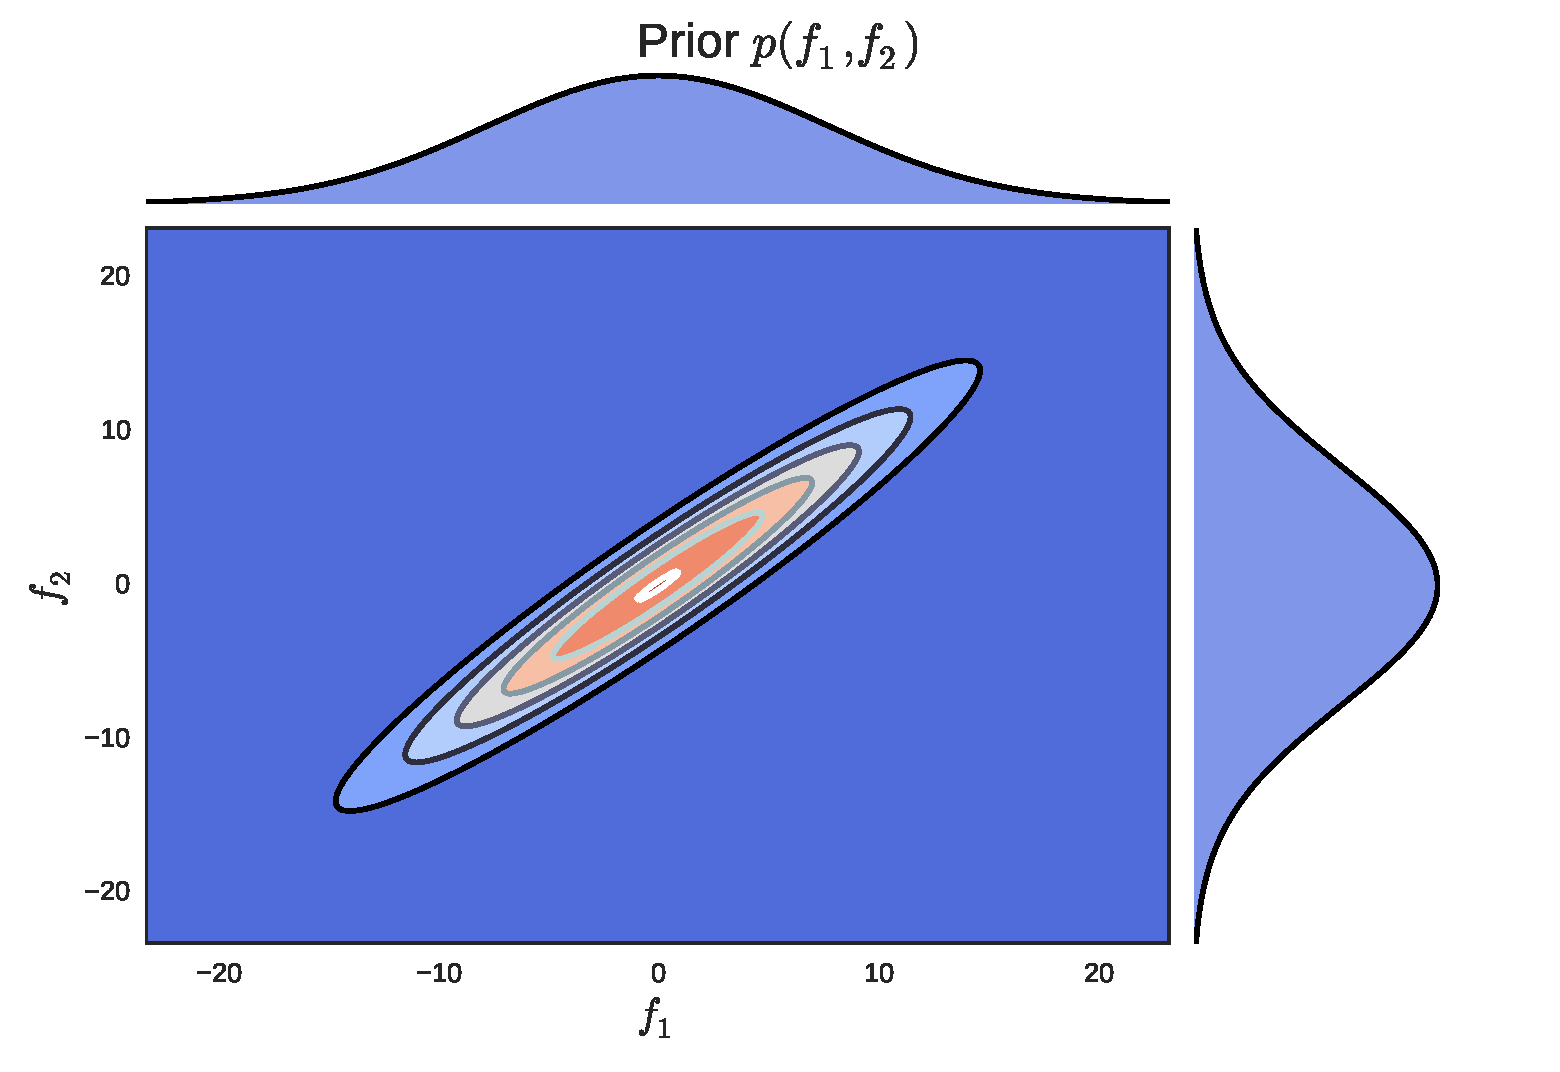
\includegraphics[width=0.55\textwidth]{../diagrams/joint_prior.pdf}
            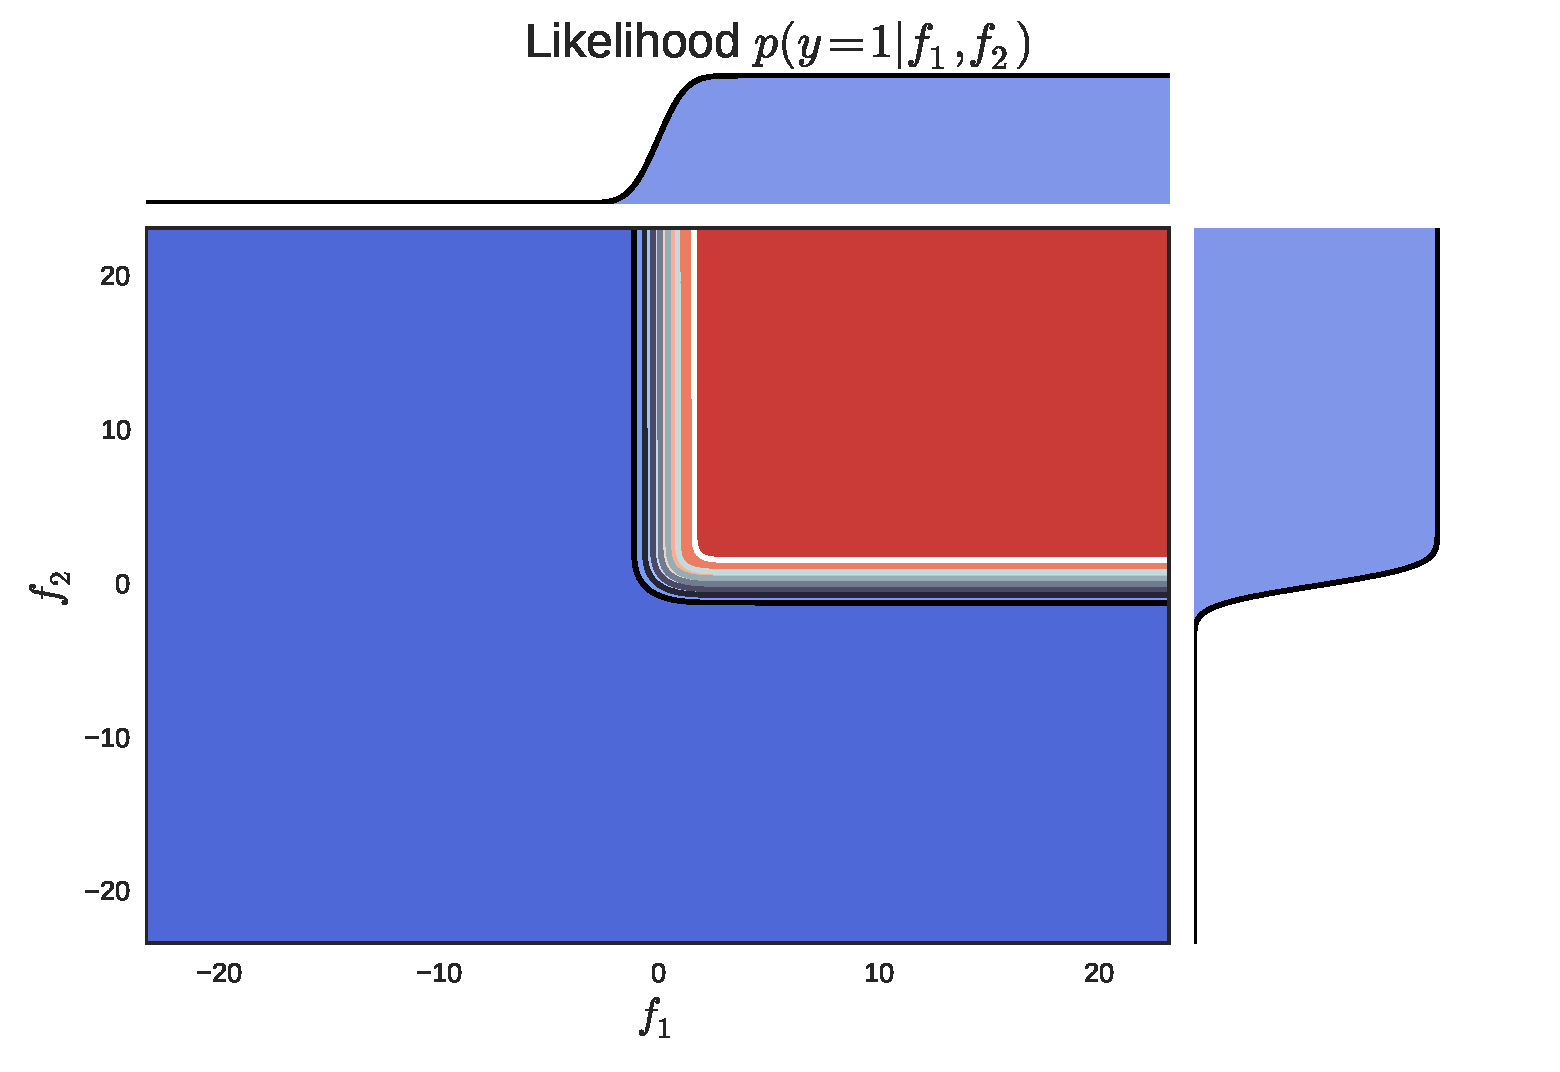
\includegraphics[width=0.55\textwidth]{../diagrams/joint_likelihood.pdf}
        }
        \onslide<2>\centerline{
            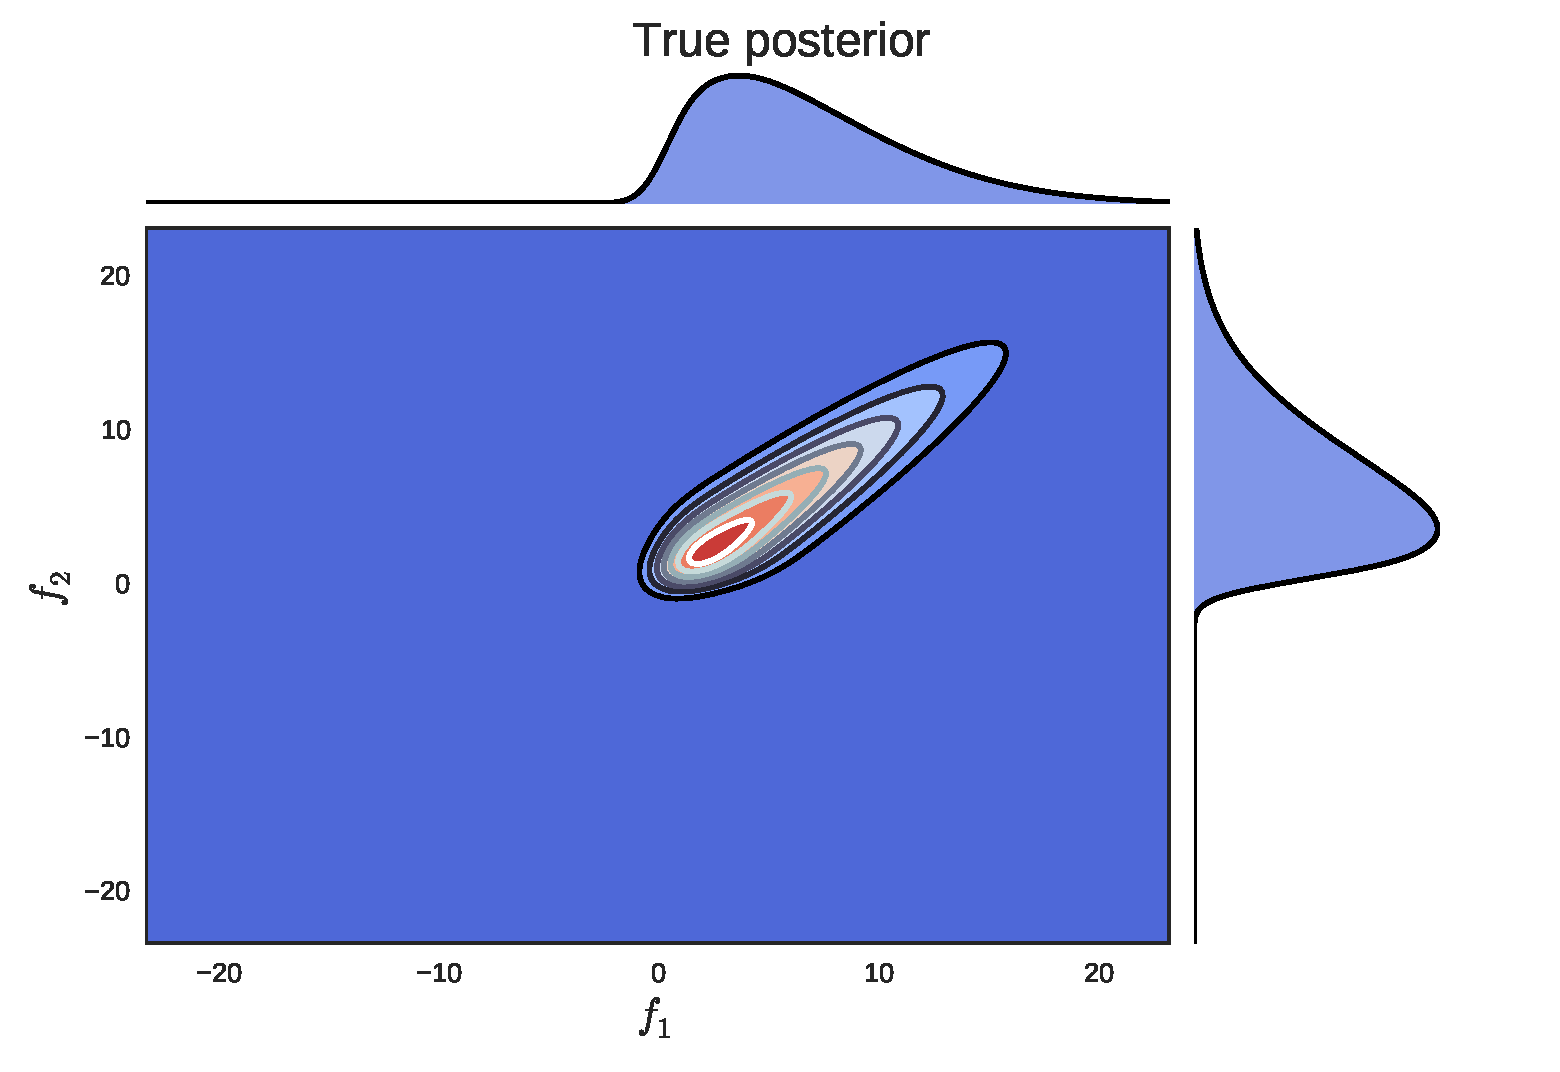
\includegraphics[width=0.55\textwidth]{../diagrams/joint_posterior.pdf}
            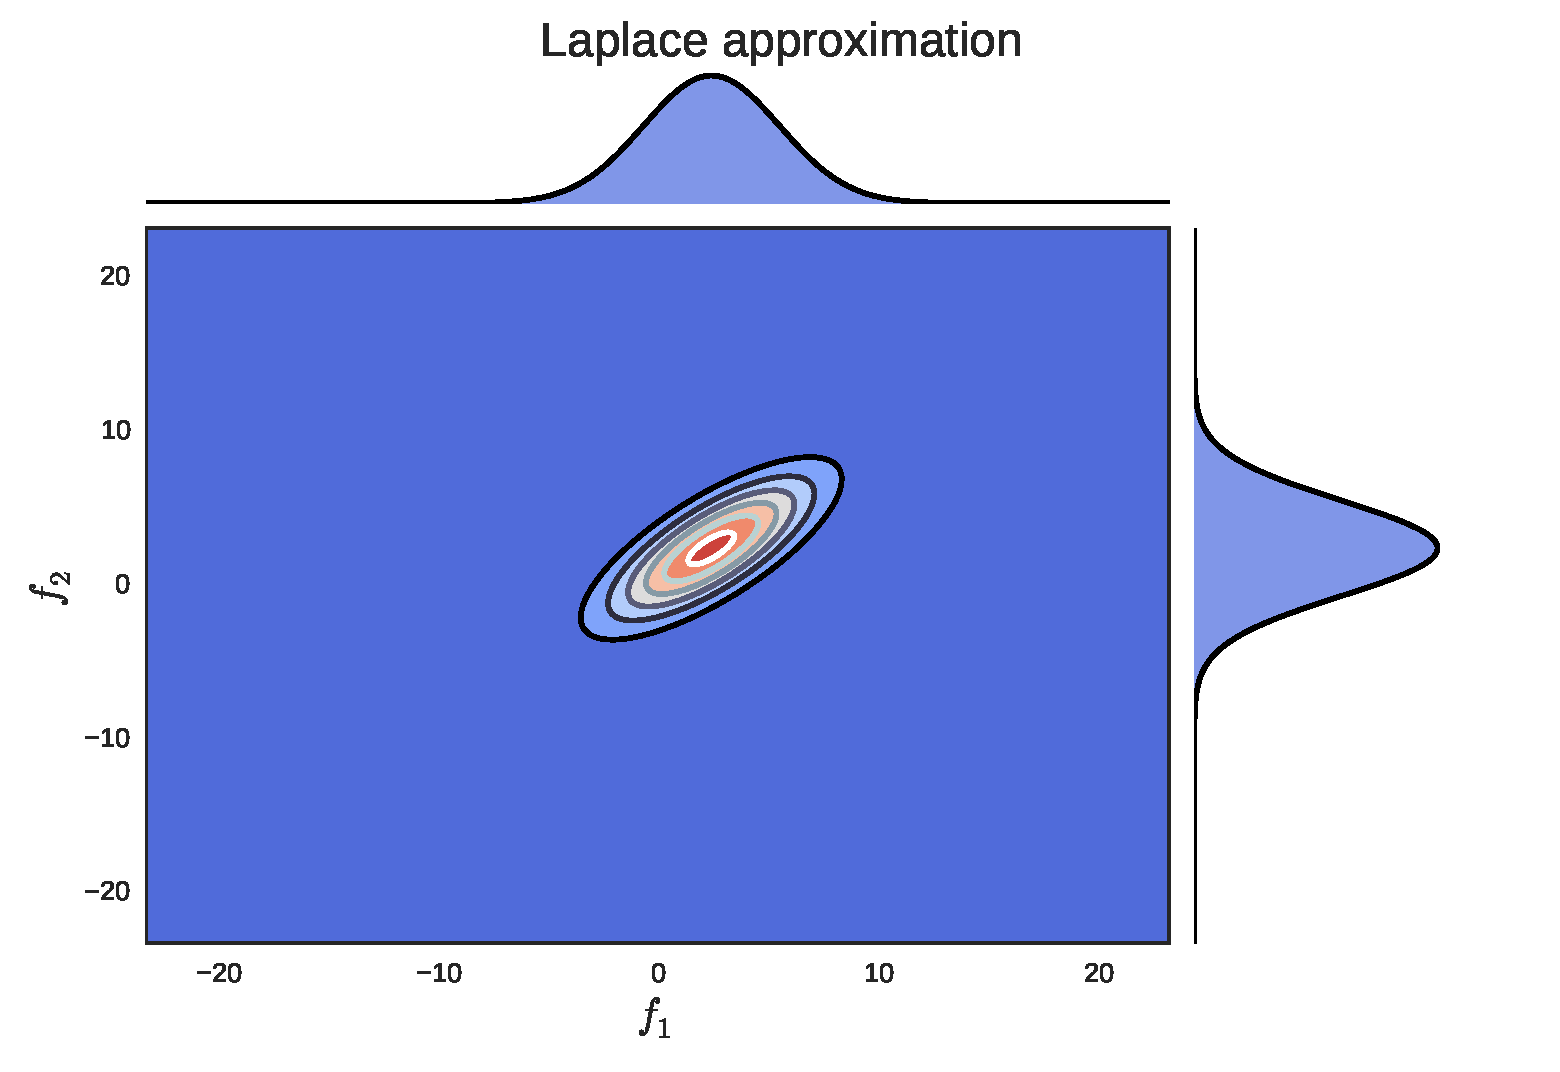
\includegraphics[width=0.55\textwidth]{../diagrams/joint_laplace.pdf}
        }
        \onslide<3>\centerline{
            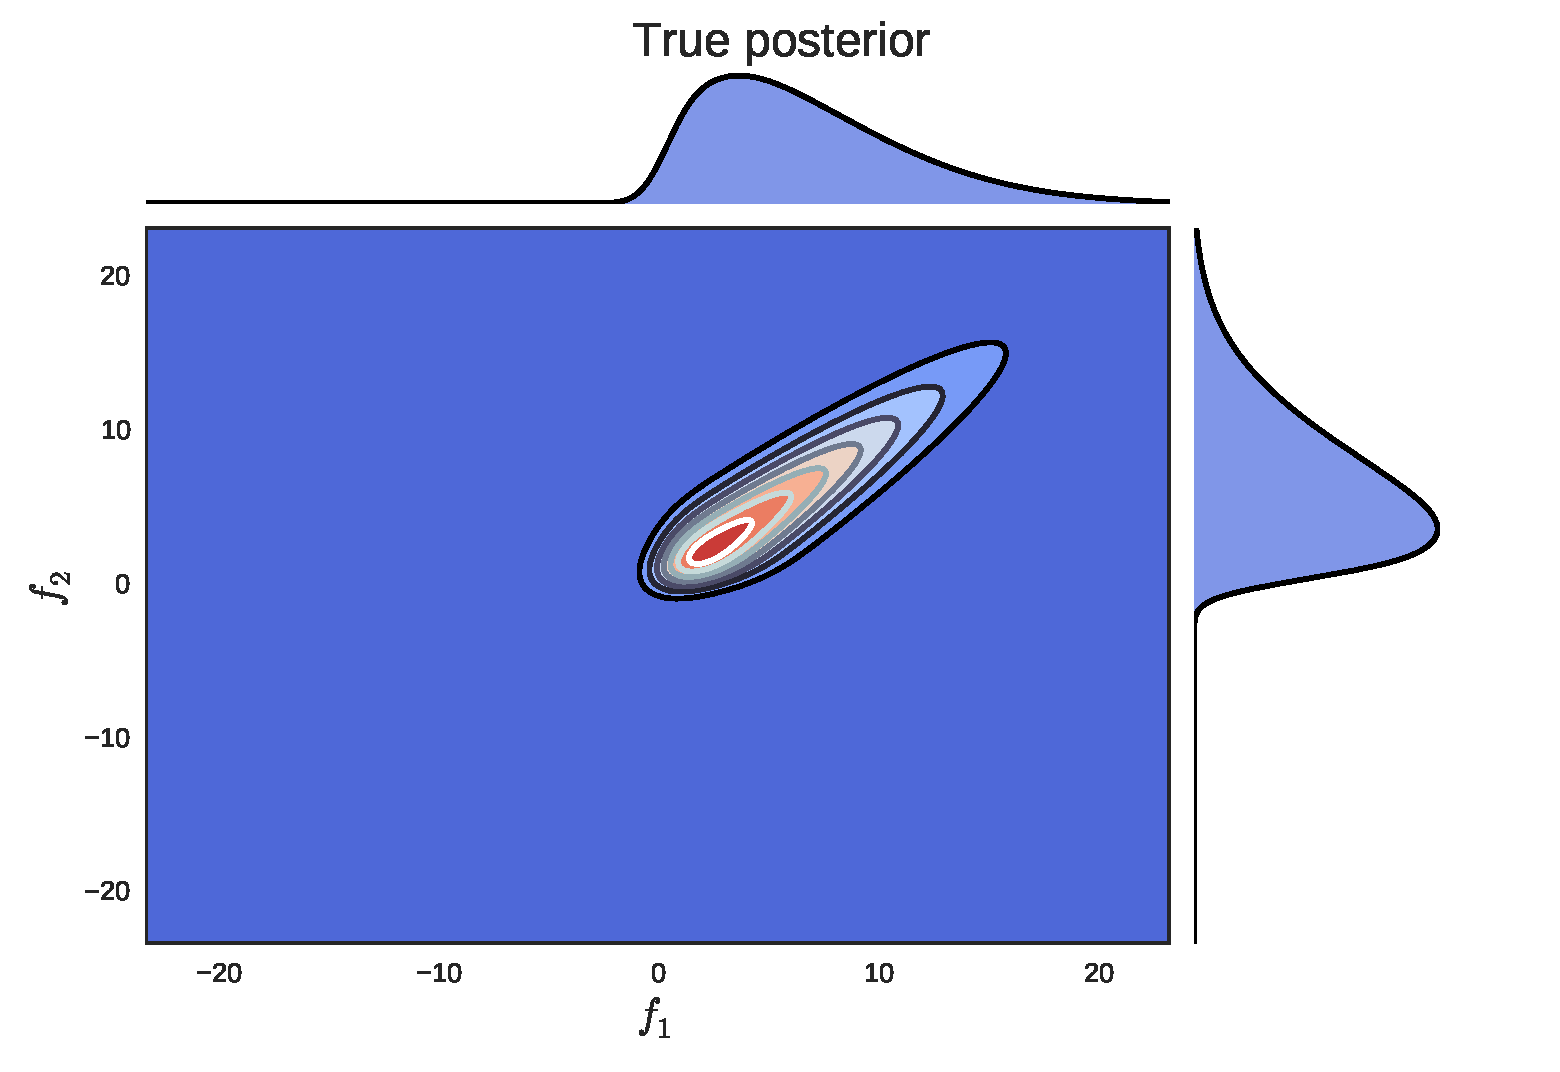
\includegraphics[width=0.55\textwidth]{../diagrams/joint_posterior.pdf}
            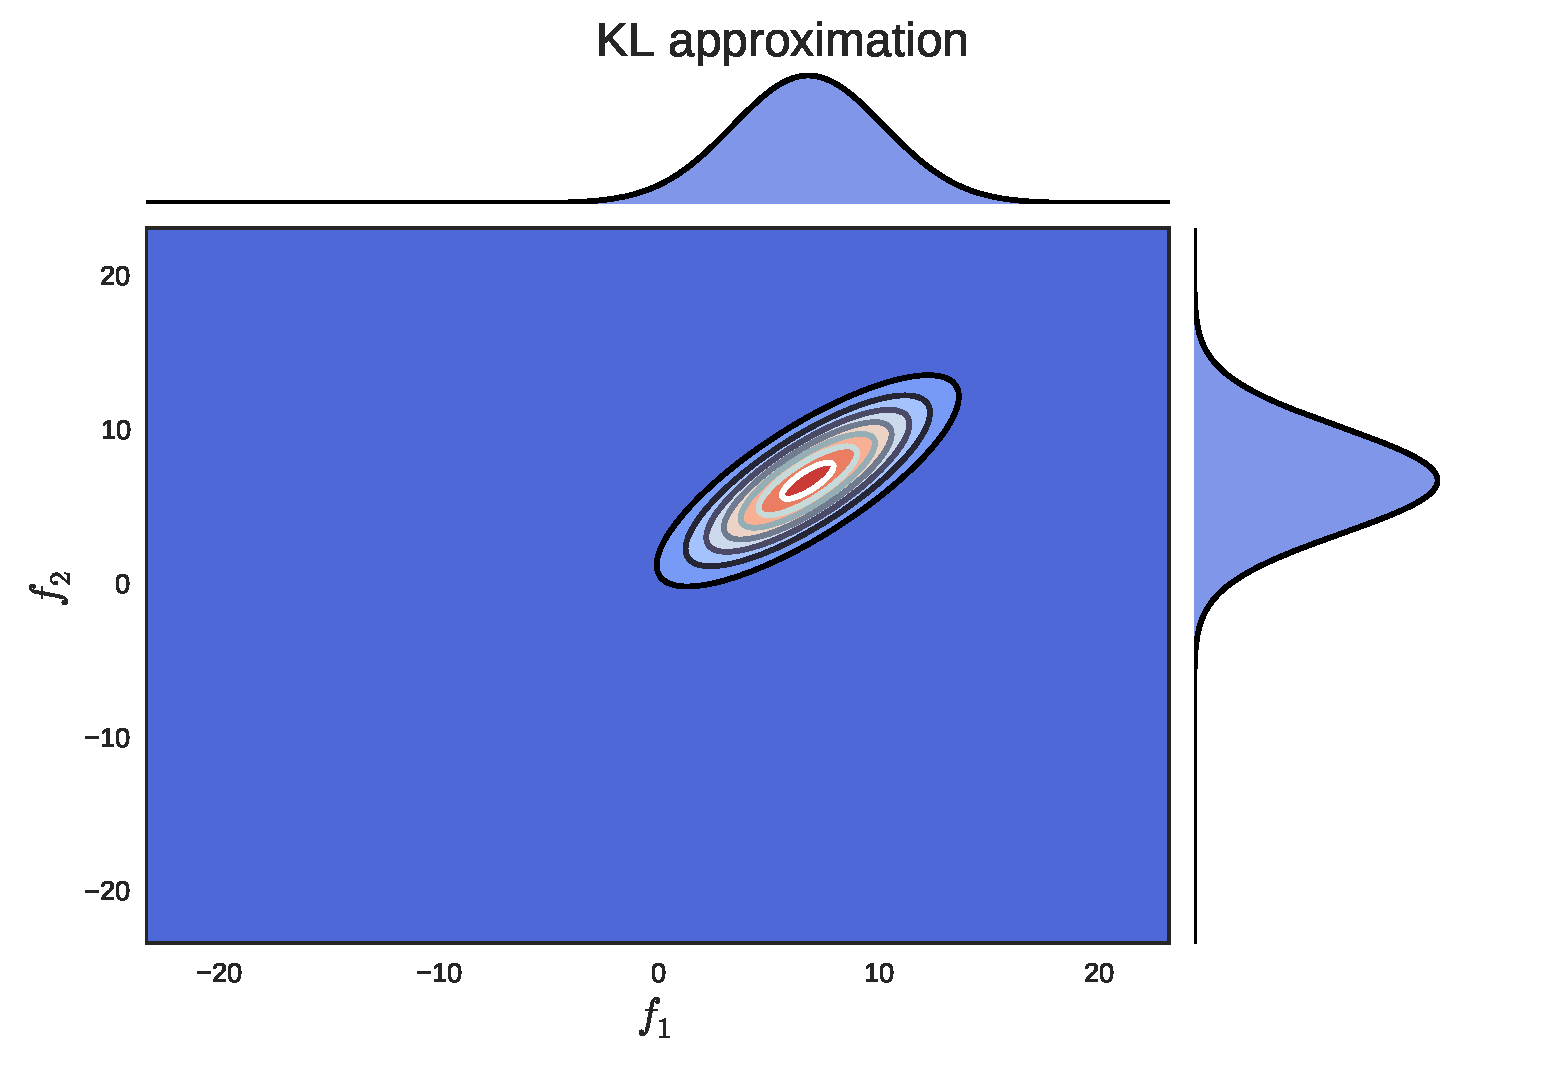
\includegraphics[width=0.55\textwidth]{../diagrams/joint_kl.pdf}
        }
        \onslide<4>\centerline{
            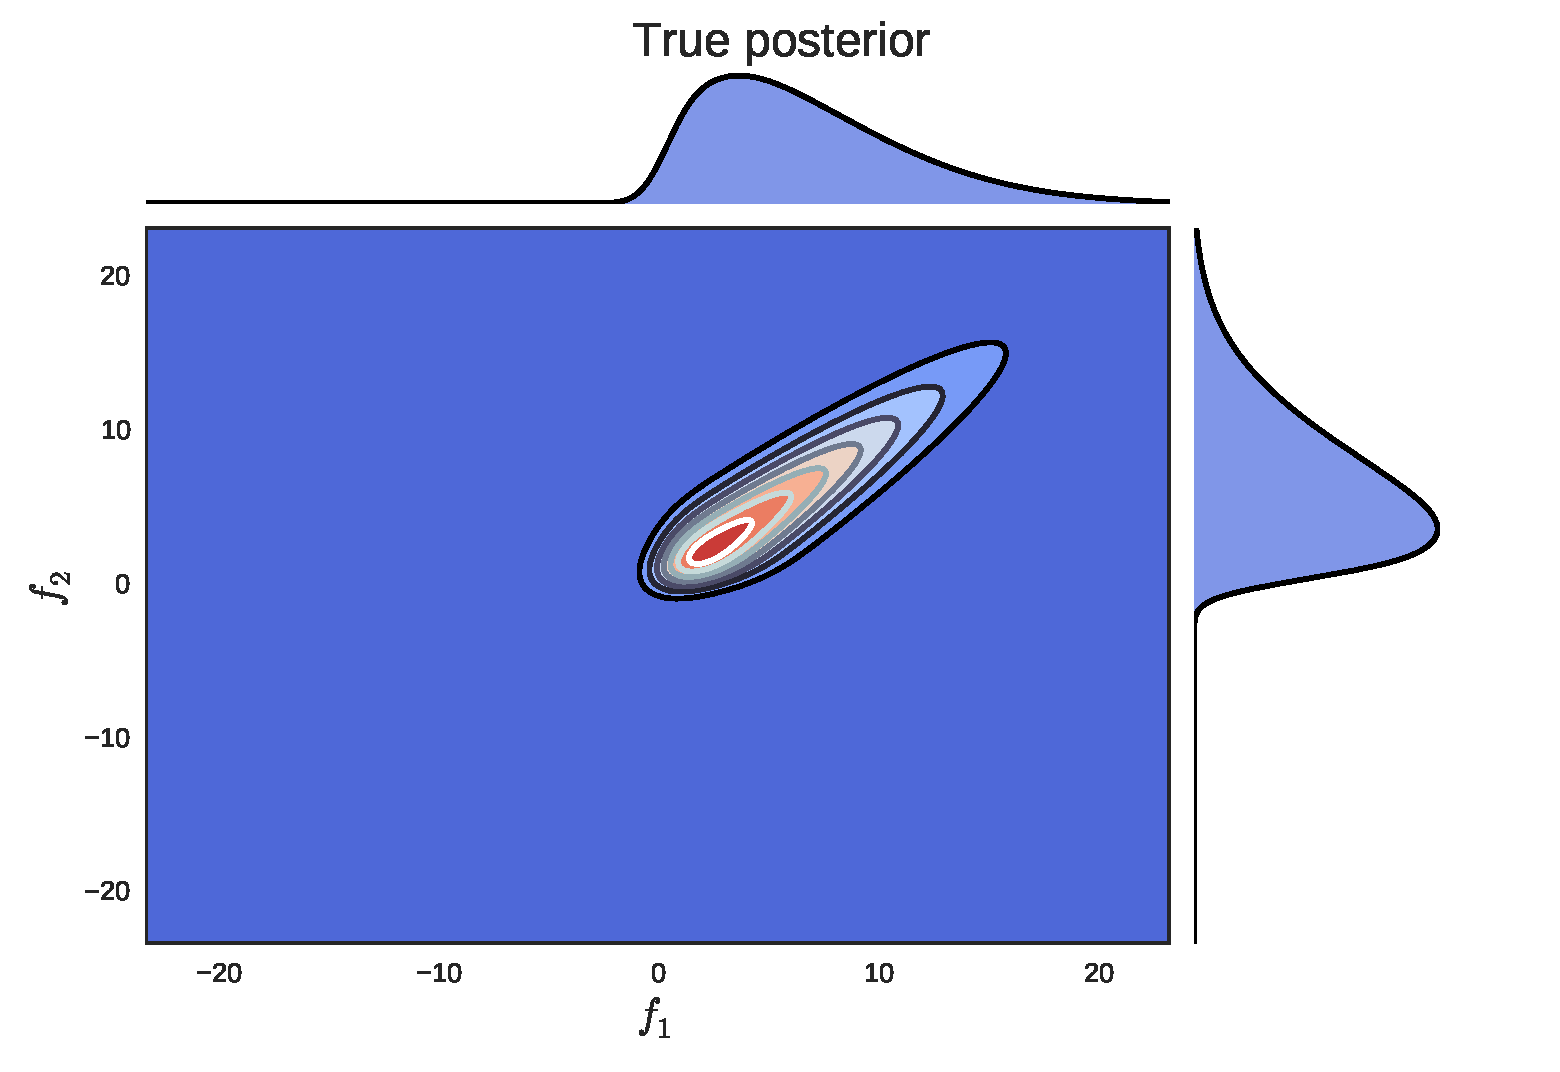
\includegraphics[width=0.55\textwidth]{../diagrams/joint_posterior.pdf}
            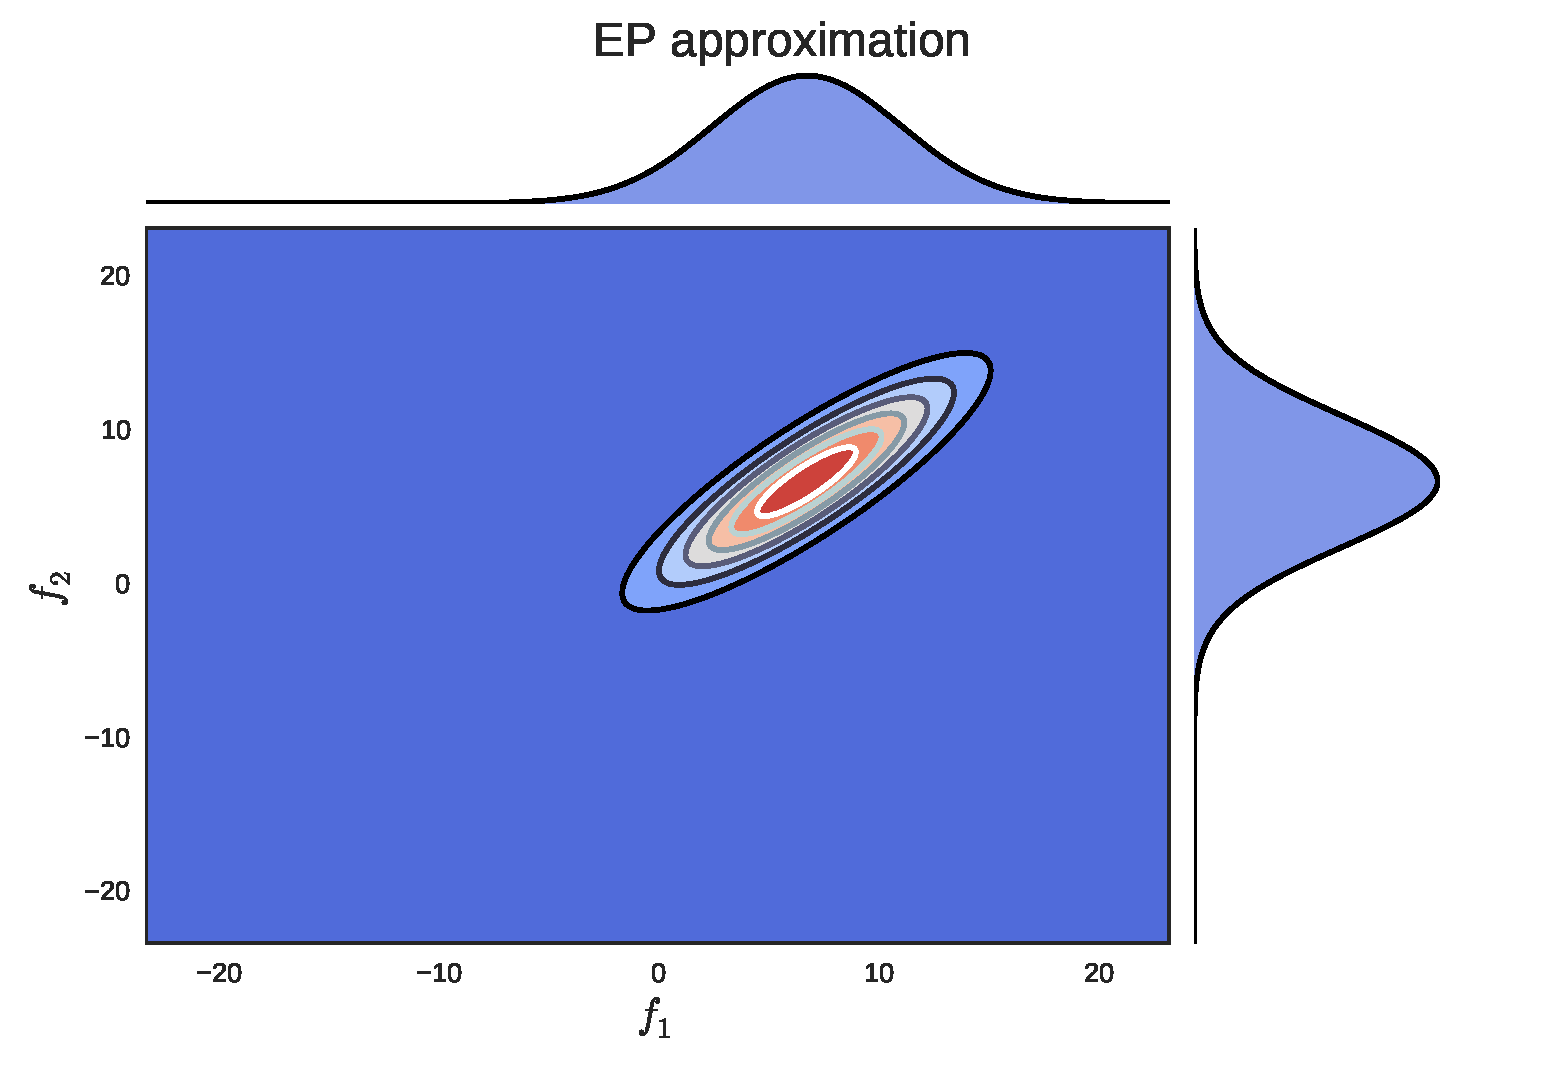
\includegraphics[width=0.55\textwidth]{../diagrams/joint_ep.pdf}
        }
    \end{overprint}
    \begin{overprint}
        \onslide<1> \begin{itemize}
            \item Gaussian prior between two function values $\{\fV_{1}, \fV_{2}\}$, at $\{\xV_{1}, \xV_{2}\}$ respectively. 
            \item Bernoulli likelihood, $\yV_{1} = 1$ and $\yV_{2} = 1$.\end{itemize}
        \onslide<2> \begin{itemize}
            \item True posterior is non-Gaussian.
            \item Laplace approximates with a Gaussian at the mode of the posterior.
        \end{itemize}
        \onslide<3> \begin{itemize}
            \item True posterior is non-Gaussian. 
            \item KL approximate with a Gaussian that has minimal KL divergence, $\KL{q(\fV)}{p(\fV|\yV)}$. 
            \item This leads to distributions that avoid regions in which $p(\fV|\yV)$ is small. 
            \item It has a large penality for assigning density where there is none.
        \end{itemize}
        \onslide<4> \begin{itemize}
            \item True posterior is non-Gaussian. 
            \item EP tends to try and put density where $p(\fV|\yV)$ is large
            \item Cares less about assigning density density where there is none. Contrasts to KL method.
        \end{itemize}
    \end{overprint}
}

\frame{
    \frametitle{Comparing posterior marginal approximations}
        \hspace{0.2em}
        \centerline{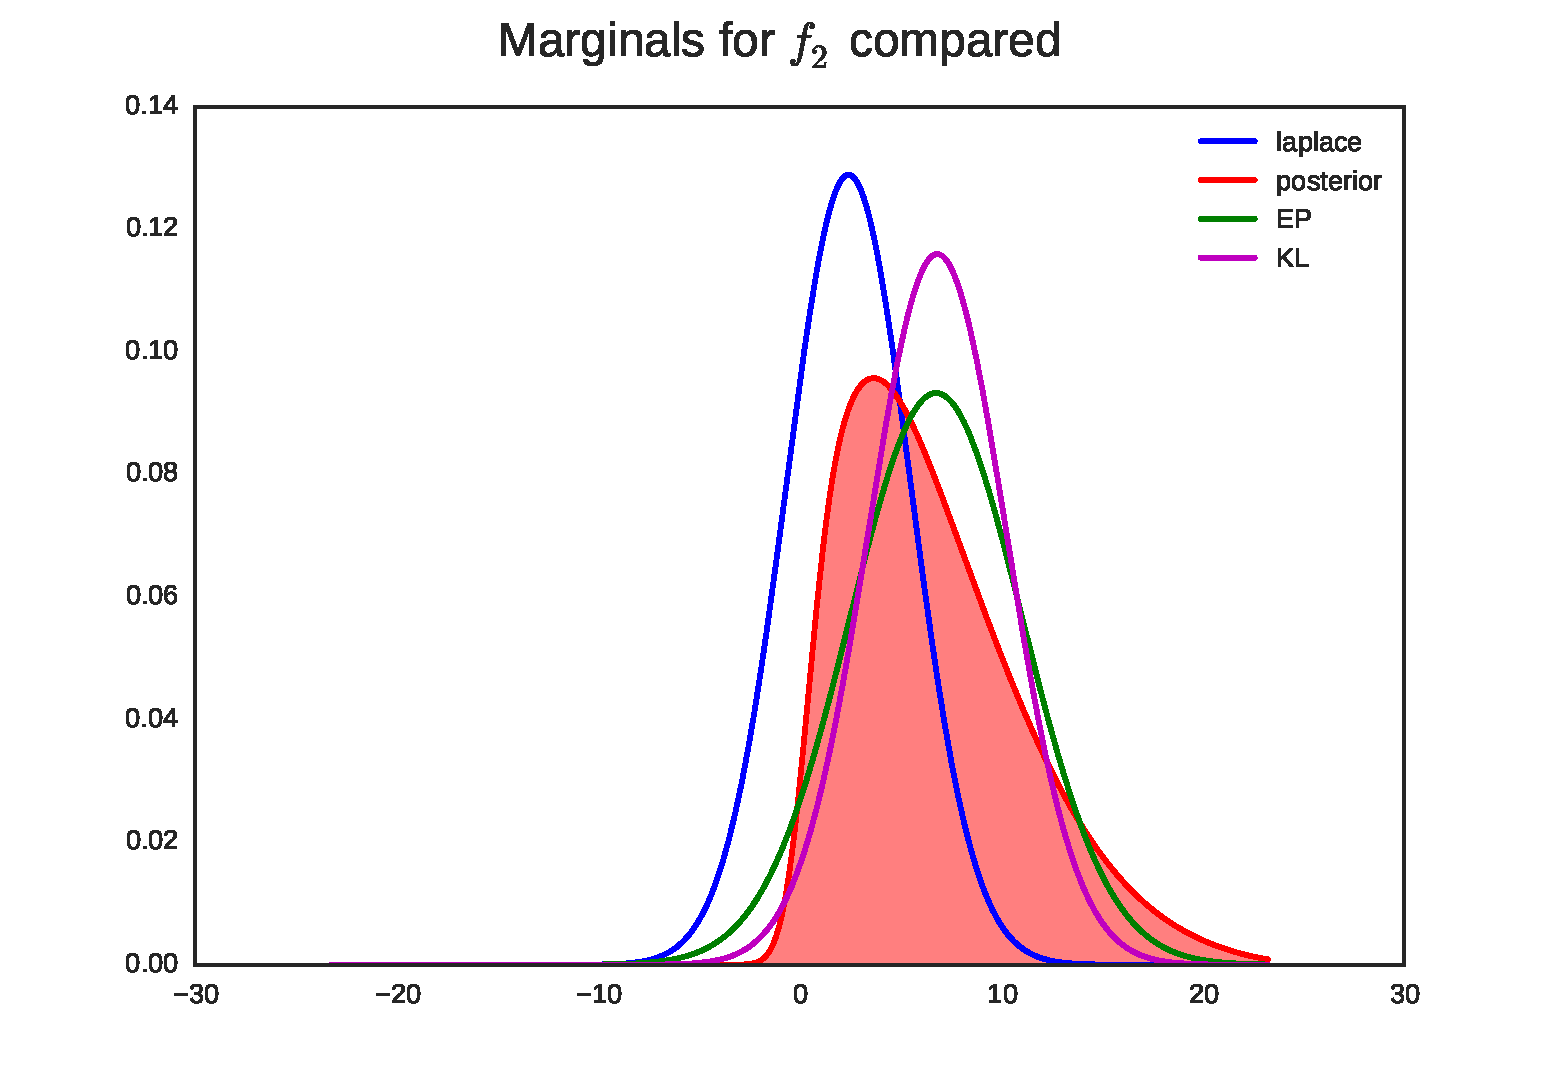
\includegraphics[width=0.7\textwidth,trim={0 1.7cm 0.5cm 0},clip]{../diagrams/marginals.pdf}}
        \hspace{-4em}
        \begin{itemize}
            \item Laplace: Poor approximation.
            \item KL: Avoids assigning density to areas where there is none, at the expense of areas where there is some (right tail).
            \item EP: Assigns density to areas with density, at the expense of areas where there is none (left tail).
        \end{itemize}
}
\frame{
    \frametitle{Pros - Cons - When - Laplace}
    Laplace approximation 
    \begin{itemize}
        \item Pros \begin{itemize}
                \item Very fast.
            \end{itemize}
        \item Cons \begin{itemize}
                \item Poor approximation if the mode does not well describe the posterior, for example Bernoulli likelihood (probit).
            \end{itemize}
        \item When \begin{itemize}
                \item When the posterior \emph{is} well characterized by its mode, for example Poisson.
            \end{itemize}
    \end{itemize}
}

\frame{
    \frametitle{Pros - Cons - When - KL}
    KL method
    \begin{itemize}
        \item Pros \begin{itemize}
                \item Principled in that it we are directly optimizing a measure of divergence between an approximation and true distribution.
                \item Can be relatively quick, and lends it self to sparse approximations~\citep{Hensman:class15}.
            \end{itemize}
        \item Cons \begin{itemize}
                \item Requires factorizing likelihoods to avoid $\numData$ dimensional integral.
                %\item Often requires numerical quadrature as part of inference, though in practice this can be very accurate.
            \end{itemize}
        \item When \begin{itemize}
                \item Likelihood is not Bernoulli, and Laplace approximation poor.
            \end{itemize}
    \end{itemize}
}

\frame{
    \frametitle{Pros - Cons - When - EP}
    EP method
    \begin{itemize}
        \item Pros \begin{itemize}
                \item Very effective for certain likelihoods (classification).
            \end{itemize}
        \item Cons \begin{itemize}
                \item Slow though possible to extend to sparse case. 
                \item Convergence issues for certain likelihoods.
                \item Must be able to match moments.
            \end{itemize}
        \item When \begin{itemize}
                \item Binary data~\citep{Nickisch:class08,Kuss:robust06}, perhaps with truncated likelihood (censored data)~\citep{Vanhatalo:gpstuff15}.
            \end{itemize}
    \end{itemize}
}

\frame{
    \frametitle{Pros - Cons - When - MCMC}
    MCMC methods
    \begin{itemize}
        \item Pros \begin{itemize}
                \item Theoretical limit gives true distribution
            \end{itemize}
        \item Cons \begin{itemize}
                \item Can be very slow
            \end{itemize}
        \item When \begin{itemize}
                \item If time is not an issue, but exact accuracy is.
                \item If you are unsure whether a different approximation is appropriate, can be used as a ``ground truth''
            \end{itemize}
    \end{itemize}
}

\frame{
    \frametitle{Questions}
    \begin{center}
        {\large Thanks for listening.\\
            \vspace{2em}Any questions?\\
        }
        \vspace{4em}
    \end{center}
}

\frame[allowframebreaks]{
    \frametitle{References}
    {\small
    \bibliography{lawrence,other,zbooks,../library}
    %\bibliography{lawrence.bib,other.bib,zbooks.bib,../library.bib}
    }
}

\end{document}
